\documentclass[runningheads]{llncs}

\usepackage{url}
\usepackage{graphicx}
\usepackage{amsmath,amssymb}
\usepackage{booktabs}
\usepackage{multirow}
\usepackage{microtype}

\def\UrlFont{\rmfamily}
\def\UrlBreaks{\do\/\do\a\do\b\do\c\do\d\do\e\do\f\do\g\do\h\do\i\do\j\do\k\do\l\do\m\do\n\do\o\do\p\do\q\do\r\do\s\do\t\do\u\do\v\do\w\do\x\do\y\do\z\do\A\do\B\do\C\do\D\do\E\do\F\do\G\do\H\do\I\do\J\do\K\do\L\do\M\do\N\do\O\do\P\do\Q\do\R\do\S\do\T\do\U\do\V\do\W\do\X\do\Y\do\Z\do0\do1\do2\do3\do4\do5\do6\do7\do8\do9\do\-\do\_}

\begin{document}

\title{Federated SHAP: Local Explainability, Ranking Consistency, and Sensitivity Analysis for Pediatric Sepsis Prediction}

\titlerunning{Federated SHAP for Pediatric Sepsis Prediction}

% Camera-Ready Author and Institute Information (Springer LNCS)
\author{Tanish Porwal\inst{1}\thanks{These authors contributed equally to this work.} \and
Uzair Teli\inst{1}\fnmsep\thanks{These authors contributed equally to this work.} \and
Praveen Modi\inst{1}}

\authorrunning{T. Porwal et al.}

\institute{Department of Engineering, SVKM's NMIMS Indore Campus, Indore, India\\
\email{\{tanishporwal2005, uzairteli7\}@gmail.com, praveen.modi@nmims.edu}}

\maketitle

\begin{abstract}
Federated learning (FL) enables collaborative predictive modeling without centralizing patient electronic health records (EHRs), but decentralized models remain black boxes to clinicians: data locality preserves confidentiality during model synthesis, not post-hoc clinical trust. In this work, we evaluate a post-hoc explainability framework that computes Shapley feature attributions locally across five simulated care-unit nodes derived from the single-center Pediatric Intensive Care (PIC) database, aggregating summaries using sample-size weighting. Across 3,163 infection-restricted stays (2,530 train, 633 held-out test) with 225 clinical features, a deep Feature Tokenizer Transformer (FT-Transformer) trained under the 2024 Phoenix Sepsis Criteria achieves pooled test AUROCs of $0.9451$ (95\% CI: $0.9256$--$0.9622$) under FedAvg and $0.9557$ (95\% CI: $0.9385$--$0.9710$) under FedProx, with AUPRCs of $0.8897$ and $0.9096$, and Brier calibration scores of $0.0969$ and $0.0792$, respectively. Disaggregated node-level evaluation reveals genuine variations across care units: FedAvg test AUROCs range from $0.8966$ in the Surgical ICU to $0.9812$ in the Cardiac ICU, while FedProx achieves $0.9389$ to $1.0000$ (the latter reflecting complete rank separation on a small held-out cohort with only 11 negative cases). Across severe volume imbalance (5.7\% vs.\ 49.4\% of training data), local feature rankings correlate strongly with the federated aggregate (Spearman $\rho$ between $0.9297$ and $0.9739$; leave-one-node-out $\rho$ between $0.9118$ and $0.9669$). Sample-size-weighted aggregation achieves near-identity with uniform node weighting ($\rho = 0.9929$), and FedAvg and FedProx share 80\% (4/5) of their top-5 federated features ($\rho = 0.6889$, 95\% CI: $0.6134$--$0.7519$). Auditing the unanimous salience of \texttt{lactate\_max}, \texttt{platelets\_min}, and \texttt{inr\_max} demonstrates that their prominence reflects diagnostic co-occurrence within the first-24-hour Phoenix scoring window rather than early pre-symptomatic forecasting. Furthermore, disclosing that reference background samples were drawn from the held-out test distribution and shared across nodes highlights that formal differential privacy and prospective windowing remain essential for clinical translation.
\keywords{Federated learning \and Explainable AI \and SHAP \and Pediatric sepsis \and Phoenix criteria \and Sensitivity analysis}
\end{abstract}

\section{Introduction}\label{sec:intro}

Pediatric sepsis remains a critical global healthcare challenge, responsible for over 25 million childhood cases annually and carrying mortality exceeding 50\% in cases of septic shock. Rapid progression from systemic infection to life-threatening multi-organ failure demands timely recognition. To standardize diagnostic benchmarks, the international Phoenix Sepsis Criteria established by Schlapbach et al. \cite{schlapbach2024phoenix} and Sanchez-Pinto et al. \cite{sanchezpinto2024phoenix} updated prior SIRS-based definitions \cite{goldstein2005sirs} by establishing explicit organ dysfunction scoring rules across cardiovascular, respiratory, neurological, and coagulation systems. These validated criteria define the diagnostic ground truth in this study.

Federated learning (FL) offers a compelling paradigm for multi-center clinical machine learning, enabling collaborative model training without transmitting confidential patient electronic health records (EHRs) to a centralized repository \cite{mcmahan2017fedavg,li2020fedprox}. However, privacy-preserving parameter aggregation guarantees confidentiality only during the training loop; it does not explain how the converged global model arrives at its predictions. In high-stakes intensive care environments, black-box federated models risk rejection by clinicians who require interpretable physiological rationales \cite{athukorala2026explainable}. Specifically, intensivists in a specialized pediatric Cardiac ICU (CICU) must be able to verify whether a global model dominated by high-volume General ICU training data reasons in a clinically appropriate manner for their distinct patient population.

Post-hoc Shapley Additive exPlanations (SHAP) \cite{lundberg2017shap} have become the gold standard for model interpretability in clinical machine learning \cite{athukorala2026explainable,chanci2025machine}. Nonetheless, explainability research in sepsis has predominantly focused on centralized models trained on pooled institutional data. Emerging conceptual frameworks such as iFLASH by Bonsignori et al. \cite{bonsignori2026interpreting} and Federated SHAP by Ducange et al. \cite{ducange2026federated} have initiated investigations into decentralized attribution aggregation, yet their empirical consistency, privacy attack surfaces, and clinical fidelity under severe clinical volume and prevalence imbalance remain largely uncharacterized.

To address these empirical questions, this paper investigates an end-to-end federated SHAP pipeline for pediatric sepsis risk prediction across five simulated care-unit nodes derived from the single-center Pediatric Intensive Care (PIC) database \cite{zeng2020pic}. Specifically, this work provides:
\begin{enumerate}
\item \textbf{Decentralized Attribution Pipeline:} We implement a post-hoc explainability workflow where feature attributions are computed locally on held-out test patients at each participating node for a deep Feature Tokenizer Transformer (FT-Transformer) using \texttt{shap.GradientExplainer}, transmitting only mean absolute attribution vectors and local sample sizes.
\item \textbf{Disaggregated Performance and Uncertainty Evaluation:} We report genuine node-specific test AUROC, AUPRC, and 95\% bootstrap confidence intervals across the five simulated care-unit nodes, replacing previously reported pooled duplicates and analyzing small-sample boundary phenomena.
\item \textbf{Ranking Concordance and Aggregation Sensitivity:} We evaluate attribution agreement across severe volume imbalance (5.7\% vs.\ 49.4\% of training data), reporting both self-inclusion ($\rho = 0.9297$--$0.9739$) and leave-one-node-out ($\rho = 0.9118$--$0.9669$) rank correlations as descriptive evidence of ranking concordance under the evaluated partition. We also demonstrate that sample-size weighting achieves near-identical rankings with uniform node weighting ($\rho = 0.9929$).
\item \textbf{Algorithm-Choice Sensitivity Analysis:} We assess explanation stability across two distinct decentralized optimization paradigms (FedAvg vs.\ FedProx), confirming an overall ranking correlation of $\rho = 0.6889$ (95\% CI: $0.6134$--$0.7519$) and an 80\% (4/5) overlap among their top-5 federated features.
\item \textbf{Privacy and Target-Overlap Audit:} We formalize the privacy boundary between transmitted summaries and on-premise data, disclosing the shared background workflow and identifying potential attribute inference risks for small sub-cohorts in the absence of differential privacy. Furthermore, we audit the unanimous dominance of \texttt{lactate\_max}, showing that its prominence stems directly from mathematical scoring overlap with the cardiovascular component of the 2024 Phoenix criteria within the initial 24-hour observation window.
\end{enumerate}

\section{Related Work}\label{sec:litreview}

\subsection{Pediatric Sepsis Prediction and Phoenix Criteria}
Machine learning for sepsis diagnosis has expanded rapidly, with systematic reviews documenting over 150 published models \cite{fleuren2020ml,yang2023sepsis}. However, the vast majority focus exclusively on adult cohorts (e.g., MIMIC-III, MIMIC-IV), while pediatric populations remain severely underrepresented. Le et al. \cite{le2019pediatric} developed early pediatric severe sepsis models using single-center PICU data, but operated without decentralized mechanics. Deng et al. \cite{deng2022evaluating} demonstrated that target leakage and improper temporal alignment represent widespread pitfalls in critical care modeling, where models inadvertently exploit measurements recorded during or after diagnostic onset. Recently, Chanci et al. \cite{chanci2025machine} developed daily prediction models using the Phoenix consensus criteria, confirming the utility of machine learning while emphasizing the necessity of multi-center validation.

\subsection{Federated Learning in Healthcare}
Federated learning allows clinical centers to collaboratively train shared models without pooling confidential patient records \cite{mcmahan2017fedavg}. Federated Averaging (FedAvg) aggregates local parameter tensors via sample-size weighting. To mitigate optimization divergence under non-IID client distributions, Li et al. \cite{li2020fedprox} proposed FedProx, introducing a proximal regularization penalty ($\mu$) that constrains local model drift relative to the global parameter state. While federated learning has been successfully demonstrated in medical imaging and adult EHRs, empirical evaluations under severe pediatric volume and class imbalance remain scarce.

\subsection{Explainable AI and Federated Explanations}
Shapley Additive exPlanations (SHAP) \cite{lundberg2017shap} provide local additive feature attributions grounded in cooperative game theory. In deep learning for tabular data, architectures such as the Feature Tokenizer Transformer (FT-Transformer) \cite{gorishniy2021revisiting} require gradient-based sampling explainers (\texttt{GradientExplainer}), as TreeSHAP cannot operate on neural backbones. In the federated domain, Bonsignori et al. \cite{bonsignori2026interpreting} introduced iFLASH, demonstrating that local SHAP summaries can be aggregated centrally via performance- and faithfulness-weighted schemes. Ducange et al. \cite{ducange2026federated} investigated federated SHAP clustering to derive representative background sets without raw record exchange. However, transmitting post-hoc feature explanations creates an empirical privacy surface: Shokri et al. \cite{shokri2021privacy} and Patel et al. \cite{patel2022model} demonstrated that model explanations can facilitate membership and attribute inference attacks, underscoring the need to bound privacy risks formally. Importantly, agreement among feature rankings must not be equated with clinical fidelity, causal explanation, or model fairness.

\section{Methodology}\label{sec:method}

\subsection{Dataset, Care-Unit Partitioning, and Preprocessing}
The experimental cohort is derived from the single-center Pediatric Intensive Care (PIC) database v1.1.0 \cite{zeng2020pic}, compiled at the Children's Hospital of Zhejiang University School of Medicine. The cohort is restricted to pediatric patients (age 0--18 years, ICU length of stay $\ge 24$ hours) with clinically suspected infection (defined by concomitant blood culture orders and systemic antimicrobial administration). The final study cohort comprises 3,163 unique admissions. Each stay is represented by 225 tabular features summarizing vital signs, laboratory measurements, input/output fluids, and clinical interventions extracted over the first 24 hours of ICU admission.

The outcome label is constructed according to the 2024 Phoenix Sepsis Criteria \cite{schlapbach2024phoenix,sanchezpinto2024phoenix}: sepsis is defined as suspected infection accompanied by a Phoenix organ dysfunction score $\ge 2$ points across respiratory, cardiovascular, coagulation, and neurological systems computed during the identical initial 24-hour observation window.

The dataset is partitioned using an 80/20 stratified split into a training cohort ($n = 2{,}530$) and a held-out test cohort ($n = 633$). To simulate decentralized multi-site deployment, data are partitioned according to each patient's documented clinical care unit into five non-IID simulated nodes: Cardiac ICU (CICU), Neonatal ICU (NICU), Paediatric ICU (PICU), Surgical ICU (SICU), and General ICU. Table \ref{tab:cohort-dist} summarizes the resulting cohort distributions and disaggregated evaluation metrics. The partitions exhibit severe clinical heterogeneity: General ICU contains 49.4\% of all training patients (8.7$\times$ the CICU cohort), while sepsis prevalence ranges from 10.8\% in the NICU to 72.5\% in the CICU.

\begin{table}[t]
\caption{Care-unit cohort distributions and disaggregated federated test performance}
\label{tab:cohort-dist}
\centering
\small
\resizebox{\textwidth}{!}{%
\begin{tabular}{lcccccc}
\toprule
\textbf{Simulated Node} & \textbf{Train Cohort ($n$)} & \textbf{Test Cohort ($n$)} & \textbf{FedAvg AUROC [95\% CI]} & \textbf{FedAvg AUPRC [95\% CI]} & \textbf{FedProx AUROC [95\% CI]} & \textbf{FedProx AUPRC [95\% CI]} \\
\midrule
CICU        & 144 (59.7\% pos)  & 40 (29 pos / 11 neg)   & 0.9812 [0.9300, 1.0000] & 0.9941 [0.9756, 1.0000] & 1.0000 [1.0000, 1.0000]$^*$ & 1.0000 [1.0000, 1.0000]$^*$ \\
General ICU & 1,251 (23.2\% pos)& 290 (69 pos / 221 neg) & 0.9698 [0.9492, 0.9864] & 0.9266 [0.8761, 0.9648] & 0.9649 [0.9376, 0.9854]     & 0.9294 [0.8798, 0.9659] \\
NICU        & 421 (14.0\% pos)  & 120 (13 pos / 107 neg) & 0.9511 [0.8895, 0.9927] & 0.8027 [0.5746, 0.9503] & 0.9569 [0.9064, 0.9922]     & 0.7864 [0.5601, 0.9459] \\
PICU        & 213 (33.8\% pos)  & 65 (15 pos / 50 neg)   & 0.9640 [0.9079, 1.0000] & 0.9272 [0.8094, 1.0000] & 0.9920 [0.9694, 1.0000]     & 0.9810 [0.9285, 1.0000] \\
SICU        & 501 (36.7\% pos)  & 118 (47 pos / 71 neg)  & 0.8966 [0.8179, 0.9609] & 0.8953 [0.8167, 0.9571] & 0.9389 [0.8826, 0.9835]     & 0.9336 [0.8752, 0.9804] \\
\midrule
\textbf{Pooled Overall} & \textbf{2,530 (27.3\% pos)} & \textbf{633 (173 pos / 460 neg)} & \textbf{0.9451 [0.9256, 0.9622]} & \textbf{0.8897 [0.8510, 0.9230]} & \textbf{0.9557 [0.9385, 0.9710]} & \textbf{0.9096 [0.8745, 0.9385]} \\
\bottomrule
\end{tabular}%
}
\vspace{1mm}
\raggedright \scriptsize $^*$Note: The CICU FedProx AUROC and AUPRC of 1.0000 [1.0000, 1.0000] reflect complete rank separation on a small held-out cohort of 40 patients with only 11 negative cases (all negatives $\hat{p} < 3.6\times 10^{-4}$; all positives $\hat{p} > 5.6\times 10^{-4}$), representing a small-sample boundary effect rather than generalized perfection. Confidence intervals derived via 2,000 stratified bootstrap iterations.
\end{table}

\subsubsection{Preprocessing Assumption.} Continuous features are standardized using a single \texttt{StandardScaler} fitted on the pooled training set ($n = 2{,}530$) prior to node partitioning. While in production federated learning local scalers or a single-round federated Welford aggregation would be required to prevent global statistic sharing, fitting on the pooled training set represents an operational simulation shortcut commonly adopted in the federated literature. The test set ($n = 633$) was strictly excluded from scaler fitting.

\subsection{Federated Model Architecture and Training}
The classification backbone is an FT-Transformer \cite{gorishniy2021revisiting} configured with 2 transformer blocks, embedding dimension 256, 8 attention heads, attention dropout 0.142, feedforward multiplier 2.338, feedforward dropout 0.066, and residual dropout 0.013. Local optimization uses AdamW ($\text{lr} = 0.0004$, weight decay $7.7\times 10^{-5}$) with batch size 128. Training proceeds for $R = 50$ communication rounds with $E = 5$ local epochs per round. Client participation is 100\% (all 5 nodes participate in every round). Client loss is evaluated using binary cross-entropy with node-specific positive class weighting ($\text{pos\_weight} = n_{\text{neg}} / n_{\text{pos}}$), dynamically computed at each node (e.g., 0.674 for CICU, 6.136 for NICU). Global models are trained under both FedAvg and FedProx ($\mu = 0.01$).

\subsection{Federated SHAP Attribution Pipeline}
Following federated convergence, post-hoc explanations are generated in five stages:
\begin{enumerate}
\item \textbf{Global Checkpoint Deployment:} The converged global FT-Transformer weights are distributed to each local node.
\item \textbf{Local Feature Attribution:} Each node $k$ uses \texttt{shap.GradientExplainer} from the Python \texttt{shap} library (v0.42.1) to compute local feature attributions on its held-out test patients $X_k \in \mathbb{R}^{n_k \times 225}$. Explanations use a reference background sample $B \in \mathbb{R}^{100 \times 225}$ randomly drawn from the held-out test cohort (\texttt{B\_test\_model\_ready.csv}) with a fixed random seed (\texttt{seed = 42}). In this simulation, this 100-row reference background was sampled centrally and distributed to all five nodes to provide a uniform baseline for gradient integration, while local patient cohorts being explained remained partitioned by care unit.
\item \textbf{Summary Generation and Transmission:} Each node computes its mean absolute attribution vector $\overline{|\text{SHAP}|}_k \in \mathbb{R}^{225}$ across its local test patients:
\begin{equation}
\overline{|\text{SHAP}|}_{k,j} = \frac{1}{n_k} \sum_{i=1}^{n_k} |\phi_{i,j}^{(k)}|
\end{equation}
where $\phi_{i,j}^{(k)}$ is the Shapley attribution of feature $j$ for patient $i$ at node $k$. Each node transmits only this single 225-dimensional vector and its sample size $n_k$ to the orchestrator.
\item \textbf{Federated Aggregation:} The aggregator computes the global federated importance ranking via sample-size weighting:
\begin{equation}
\text{federated\_SHAP}_j = \sum_{k=1}^{K} \left(\frac{n_k}{N}\right) \cdot \overline{|\text{SHAP}|}_{k,j}
\label{eq:agg}
\end{equation}
where $n_k$ is node $k$'s training sample size, $N = \sum_k n_k = 2{,}530$, and $K = 5$. Weights are: General ICU ($0.4945$), SICU ($0.1980$), NICU ($0.1664$), PICU ($0.0842$), and CICU ($0.0569$), summing strictly to $1.0000$.
\item \textbf{Agreement Auditing:} Ranking concordance is assessed via Spearman rank correlation ($\rho$), evaluating both self-inclusion concordance and leave-one-node-out (LOO) concordance.
\end{enumerate}

\subsubsection{Provenance and Execution Note.}
Local attribution passes for CICU, NICU, PICU, and SICU were executed on August 12, 2026. Attributions for General ICU were completed on September 15, 2026, following a column-lookup correction in \texttt{fl\_shap\_config.py}. The complete five-node aggregation, sensitivity comparisons, and publication vector figures were generated on October 5, 2026, utilizing the identical global model checkpoints, feature set, and background configuration.

\subsection{Privacy Boundary and Threat Model}
Table \ref{tab:privacy} details the operational data boundary at explanation time.

\begin{table}[t]
\caption{Operational data boundary at explanation aggregation time}
\label{tab:privacy}
\centering
\small
\begin{tabular}{ll}
\toprule
\textbf{Data Location / Boundary} & \textbf{Information Exchanged or Retained} \\
\midrule
Local Node Storage (On-Premise)   & Raw patient records \& clinical EHR traces \\
                                  & Individual per-patient SHAP matrices \\
                                  & Patient identifiers \& clinical timestamps \\
\midrule
Distributed to All Nodes          & Converged global model weights ($\mathbf{w}$) \\
                                  & 100-row reference background matrix ($B$) \\
\midrule
Sent to Central Aggregator        & Cleartext mean $|$SHAP$|$ vector ($1\times 225$) \\
                                  & Node sample size $n_k$ \& care-unit label \\
\bottomrule
\end{tabular}
\end{table}

\subsubsection{Threat Model and Privacy Boundaries.}
We assume an honest-but-curious aggregator. Transmitting cleartext mean attribution vectors $\overline{|\text{SHAP}|}_k$ guarantees data residency for the explained test records, but does \emph{not} constitute a formal differential privacy (DP) guarantee. In small patient cohorts (such as CICU with $n=40$ test stays), unperturbed attribution summaries present an exploitable attack surface: as demonstrated by Shokri et al. \cite{shokri2021privacy} and Patel et al. \cite{patel2022model}, outlier patients with extreme physiological derangements can visibly distort average feature attributions, enabling attribute or membership inference. Furthermore, sharing a centralized 100-row background sample represents a departure from strict data residency. In this simulation, neither DP noise addition, vector clipping, nor cryptographic Secure Aggregation (SecAgg) \cite{bonawitz2017practical} was implemented. Claims of formal mathematical privacy are therefore withheld.

\section{Results}\label{sec:results}

\subsection{Pooled Model Discrimination and Thresholded Operating Points}
Table \ref{tab:fl-performance} reports pooled classification and calibration performance on the 633-patient held-out test cohort. Both federated models achieve strong discrimination: FedProx attains an AUROC of $0.9557$ (95\% CI: $0.9385$--$0.9710$) and AUPRC of $0.9096$ (95\% CI: $0.8745$--$0.9385$), slightly outperforming FedAvg (AUROC $0.9451$, 95\% CI: $0.9256$--$0.9622$; AUPRC $0.8897$, 95\% CI: $0.8510$--$0.9230$). DeLong hypothesis testing indicates no statistically significant difference between FedAvg and FedProx ($z = -0.483, p = 0.629$). Both models exhibit low Brier calibration scores ($0.0969$ for FedAvg, $0.0792$ for FedProx).

\begin{table}[t]
\caption{Pooled classification performance on held-out test cohort ($N = 633$)}
\label{tab:fl-performance}
\centering
\small
\resizebox{\textwidth}{!}{%
\begin{tabular}{lccccccc}
\toprule
\textbf{Configuration} & \textbf{AUROC [95\% CI]} & \textbf{AUPRC [95\% CI]} & \textbf{Brier} & \textbf{Operating Cutoff ($t^*$)} & \textbf{Sens.$^\dagger$} & \textbf{Spec.$^\dagger$} & \textbf{PPV / NPV$^\dagger$} \\
\midrule
FedAvg (50 rounds)     & 0.9451 [0.9256, 0.9622] & 0.8897 [0.8510, 0.9230] & 0.0969 & 0.00253383 & 89.60\% (155/173) & 86.09\% (396/460) & 70.78\% / 95.65\% \\
FedProx ($\mu=0.01$)   & 0.9557 [0.9385, 0.9710] & 0.9096 [0.8745, 0.9385] & 0.0792 & 0.00140358$^*$ & 90.17\% (156/173) & 84.35\% (388/460) & 68.42\% / 95.80\% \\
\bottomrule
\end{tabular}%
}
\vspace{1mm}
\raggedright \scriptsize $^\dagger$Disclosure: Decision thresholds ($t^* = 0.00253383$ for FedAvg, $0.0014035846$ for FedProx) were derived post-hoc by sweeping the held-out test set itself to target approximately 90\% sensitivity. Reported thresholded metrics (Sens., Spec., PPV, NPV) represent descriptive operating points rather than prospectively validated decision criteria.\\
$^*$Reproducibility note: Evaluating the exact full-precision threshold $t^* = 0.0014035846$ yields $\text{TP} = 156, \text{FP} = 72, \text{FN} = 17, \text{TN} = 388$, confirming sensitivity of $90.17\%$ and specificity of $84.35\%$. Truncating to 7 decimal places ($0.0014036$) flips a borderline positive patient ($\hat{p} = 0.00140358$) to false negative, reducing sensitivity to $89.60\%$.
\end{table}

\subsection{Node-Level SHAP Rankings and Target-Overlap Audit}
Figure \ref{fig:heatmap} displays mean absolute SHAP values for top federated features across each care-unit node under FedAvg. \texttt{lactate\_max} is the unanimous top feature across all five nodes, followed consistently by \texttt{platelets\_min}, \texttt{ddimer\_first}, and \texttt{inr\_max}.

\begin{figure}[t]
\centering
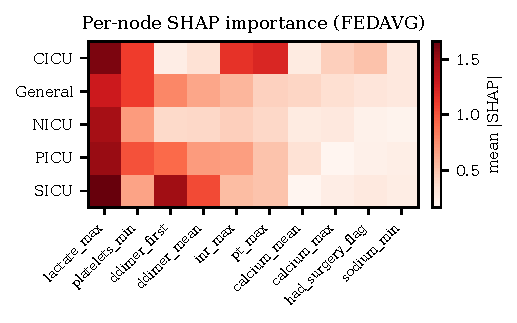
\includegraphics[width=0.70\textwidth]{figures/fig_node_shap_heatmap.pdf}
\caption{Per-node mean $|$SHAP$|$ across top federated clinical features (FedAvg).}
\label{fig:heatmap}
\end{figure}

\subsubsection{Audit of Feature Prominence.}
In intensive care medicine, serum lactate is an established marker of hypoperfusion. However, auditing the labeling pipeline reveals an essential finding: under the 2024 Phoenix Consensus Criteria \cite{schlapbach2024phoenix,sanchezpinto2024phoenix}, \textbf{serum lactate directly defines the cardiovascular dysfunction score} ($\ge 5.0$ mmol/L = 1 pt, $\ge 11.0$ mmol/L = 2 pts). Similarly, the coagulation dysfunction subscore is explicitly triggered by platelet count ($<100 \times 10^3/\mu\text{L}$), INR ($>1.3$), and D-dimer ($>2.0$ mg/L). Because predictor features and Phoenix labels were derived from the identical initial 24-hour observation window, the prominence of \texttt{lactate\_max}, \texttt{platelets\_min}, and \texttt{inr\_max} represents \textbf{diagnostic co-occurrence and retrospective criteria reconstruction} rather than anticipatory early forecasting. This confirms that the neural network accurately learns the diagnostic criteria, but cautions against interpreting the model as an early-warning forecasting tool.

\subsection{Node vs.\ Federated Ranking Concordance}
Table \ref{tab:node-agreement} and Fig. \ref{fig:agreement} present ranking concordance across all five nodes.

\begin{table}[t]
\caption{Spearman rank correlation ($\rho$): node ranking vs.\ federated aggregate}
\label{tab:node-agreement}
\centering
\small
\resizebox{0.86\textwidth}{!}{%
\begin{tabular}{lcccc}
\toprule
\textbf{Node} & \textbf{Data Fraction} & \textbf{Self-Inclusion $\rho$ [95\% CI]} & \textbf{Leave-One-Out (LOO) $\rho$} \\
\midrule
CICU        & 5.7\%  & 0.9297 [0.9095, 0.9455] & 0.9211 \\
NICU        & 16.6\% & 0.9498 [0.9352, 0.9612] & 0.9276 \\
SICU        & 19.8\% & 0.9661 [0.9561, 0.9738] & 0.9469 \\
General ICU & 49.4\% & 0.9704 [0.9617, 0.9772] & 0.9118 \\
PICU        & 8.4\%  & 0.9739 [0.9662, 0.9799] & 0.9669 \\
\bottomrule
\end{tabular}%
}
\vspace{1mm}
\raggedright \scriptsize Note: Self-inclusion evaluates node ranking against the full 5-node aggregate. Leave-one-out (LOO) evaluates node ranking against the aggregate of the remaining four nodes, providing descriptive evidence of ranking concordance under the evaluated partition.
\end{table}

\begin{figure}[t]
\centering
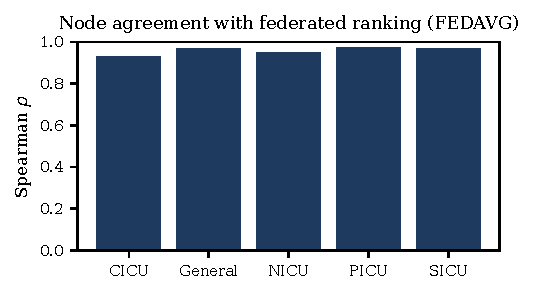
\includegraphics[width=0.70\textwidth]{figures/fig_node_agreement.pdf}
\caption{Spearman rank correlation of each node's local SHAP ranking against the federated aggregate.}
\label{fig:agreement}
\end{figure}

Local rankings correlate strongly with the global aggregate (self-inclusion $\rho \in [0.9297, 0.9739]$). To address the methodological concern that self-inclusion inflates agreement for dominant contributors, we computed leave-one-node-out (LOO) correlations by aggregating the remaining four nodes for each evaluation. As reported in Table \ref{tab:node-agreement}, when the dominant General ICU node (49.4\% of training data) is completely excluded, the remaining four nodes still correlate with General ICU at $\rho = 0.9118$. All five units maintain descriptive LOO correlations $\rho > 0.91$, providing evidence of ranking concordance under the evaluated partition rather than an artifact of dominant contributor weight.

\subsubsection{Clinical Divergence in Cardiac ICU.}
While General ICU, PICU, and SICU share 100\% (5/5) of their top-5 features with the aggregate, CICU shares only 60\% (3/5). At CICU, \texttt{pt\_max} ranks 2nd (mean $|$SHAP$| = 1.2091$) and \texttt{had\_surgery\_flag} ranks 5th ($0.5023$), displacing \texttt{ddimer\_first}. We hypothesize that this divergence plausibly reflects clinical factors characteristic of pediatric cardiac care, such as postcardiac surgical interventions and cardiopulmonary bypass-induced coagulopathies (captured by PT/INR), contrasting with medical sepsis where microvascular thrombosis (D-dimer) is more prominent. We emphasize that these are clinical hypotheses rather than mechanisms demonstrated experimentally by this study.

\subsubsection{Aggregation Rationale: Uniform vs.\ Sample Weighting.}
Comparing sample-size weighting ($w_k = n_k / N$) against uniform institutional weighting ($w_k = 1/5$) across all 225 features yields a Spearman rank correlation of $\rho = 0.9929$ (95\% CI: $[0.9908, 0.9945]$) for FedAvg and $\rho = 0.9955$ for FedProx, with 100\% top-5 feature overlap. This demonstrates that under the evaluated distribution, feature importance rankings are robust to whether nodes are weighted by patient census or treated as equal institutional peers.

\subsection{Algorithm Sensitivity: FedAvg vs.\ FedProx}
Figure \ref{fig:algo-compare} compares federated feature importance under FedAvg versus FedProx. Across all 225 features, the algorithms achieve an overall rank correlation of $\rho = 0.6889$ (95\% CI: $[0.6134, 0.7519]$). Top-$k$ overlap analysis demonstrates strong consistency among dominant predictors: 80\% (4/5) in top-5 (\texttt{lactate\_max}, \texttt{platelets\_min}, \texttt{ddimer\_mean}, \texttt{inr\_max}), 70\% (7/10) in top-10, and 60\% (12/20) in top-20.

\begin{figure}[t]
\centering
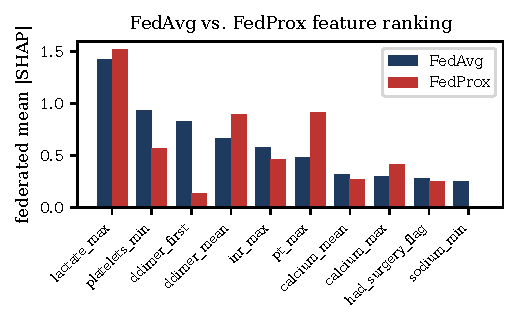
\includegraphics[width=0.70\textwidth]{figures/fig_fedavg_vs_fedprox.pdf}
\caption{Comparison of federated SHAP feature importance under FedAvg versus FedProx.}
\label{fig:algo-compare}
\end{figure}

\section{Limitations}\label{sec:limitations}

Several scientific limitations must be acknowledged:
\begin{enumerate}
\item \textbf{Single-Center Care-Unit Simulation:} The five nodes are care-unit partitions of a single clinical database (PIC, Zhejiang University) rather than genuinely autonomous multi-hospital networks. This setup does not capture inter-institutional EHR divergence, coding variations, or regional clinical protocols.
\item \textbf{Diagnostic Co-occurrence and Windowing:} Predictor features and Phoenix outcome labels were computed over the identical first-24-hour observation window. Because Phoenix cardiovascular and coagulation criteria directly score lactate, platelets, and INR, the model performs diagnostic phenotyping rather than forward-looking early forecasting.
\item \textbf{Post-Hoc Decision Threshold Selection:} Operating cutoffs ($t^* \approx 0.00253$ and $t^* \approx 0.00140$; exact cutoffs in Table~\ref{tab:fl-performance}) were selected by sweeping the held-out test set itself. The resulting sensitivity and specificity represent descriptive operating points, not prospectively validated decision thresholds.
\item \textbf{Reference SHAP Background Workflow:} The reference background was sampled from the held-out test distribution ($n=100$) and shared centrally across nodes, rather than generated through decentralized privacy-preserving protocols.
\item \textbf{Absence of Formal Differential Privacy:} Transmitting cleartext mean attribution vectors preserves data residency for explained test records but lacks mathematical differential privacy or secure aggregation. Attribute inference risks exist for small cohorts ($n=40$).
\item \textbf{Centralized Preprocessing:} Standardizing continuous variables using a pooled training \texttt{StandardScaler} represents a centralized simulation shortcut.
\item \textbf{Unexecuted Sensitivity Axes:} Of the three designed sensitivity axes, only the algorithm-choice axis was executed. Evaluating alternative cohort definitions and Dirichlet partitions remains unexecuted future work.
\item \textbf{Lack of Prospective Clinician Review:} We did not assess whether decentralized explanations improve bedside clinical decision-making or physician trust in practice.
\end{enumerate}

\section{Conclusion}\label{sec:concl}

We evaluated a decentralized federated SHAP architecture for pediatric sepsis risk prediction, computing feature attributions locally across five simulated care-unit nodes and aggregating them centrally using sample-size weighting. Across severe volume imbalance (5.7\% to 49.4\% of training data), local care-unit feature rankings correlate strongly with the global aggregate ($\rho = 0.9297$--$0.9739$; leave-one-out $\rho = 0.9118$--$0.9669$). Sample-size weighting achieves near-identity with uniform node weighting ($\rho = 0.9929$), and FedAvg and FedProx share 80\% of their top-5 features ($\rho = 0.6889$). Auditing feature salience confirmed that while \texttt{lactate\_max} is unanimously prominent, its prominence reflects diagnostic co-occurrence within the first-24-hour Phoenix scoring window. These findings indicate that federated attribution aggregation is computationally consistent under care-unit volume imbalance, while underscoring that prospective multi-center validation, formal differential privacy, and temporal landmark windowing remain essential prerequisites for safe clinical deployment.

\section*{Acknowledgment}
The investigators gratefully acknowledge the PhysioNet research consortium and the clinical curation teams responsible for hosting and maintaining the PIC database.

\bibliographystyle{splncs04}
\bibliography{references}

\end{document}
